\chapter{Proposed solutions}\label{chap:proposed_solutions}

	Motivated by previous solutions, mentioned in Chapter \ref{chap:existing_solutions}, Sections \ref{subsec:intra_inter} and \ref{subsec:linear_geo}, we propose multiple approaches to solve the problem of tracklet building. The first one, described in Section \ref{sec:linear_regression} takes advantage of the facts mentioned in Section \ref{subsec:linear_geo}, specifically that picking sufficiently small part of the object's trajectory will make the object appear as if it moved in uniform linear motion. Section \ref{sec:IDO} describes an algorithm which filters and validates data gathered in Section \ref{sec:linear_regression}. An experimental neural network's construction and relevance is discussed in Section \ref{sec:neural} and Section \ref{sec:hough} acknowledges another possible solution which has not been implemented but has been considered nevertheless.

\section{Use of linear regression}\label{sec:linear_regression}

	Linear regression is a well-known statistical concept modelling the linear relationship between a scalar dependent variable \emph{y} and one or more independent variables, usually denoted as \emph{x}. In this thesis, we will be using a single scalar predictor variable and a single scalar response variable - simple linear regression (SLR). We chose SLR because objects in our case appear as if they followed the rules of uniform linear motion (for details on uniform linear motion, see Chapter \ref{chap:existing_solutions}, Section \ref{sec:linear_motion}). For more information about linear regression as a statistical model, see \citep{freedman2005statistical}.
	
	To successfully create a tracklet, we need to have three or more confirmed observations out of several images of the same portion of the night sky. As described in Chapter \ref{chap:object_dynamics}, Section \ref{sec:proc_seg_reduc} all objects are classified beforehand and have several mandatory attributes assigned to them.
	
	As discussed in Chapter \ref{chap:object_dynamics}, Section \ref{sec:ccd} objects' position on the image reference frame in each image in the set of provided inputs (see Chapter \ref{chap:requirements}, Section \ref{sec:input_data}) are represented by the values \emph{x} and \emph{y}. The first draft of linear regression was designed and realised using these values - \emph{x} as an independent value and \emph{y} as a dependent value.
	
	There are several unidentified or misidentified objects which are potentially the object we are looking for, represented as points. 
	
	Firstly, we pair each unidentified point $p_1$ of an object $o_1$ from the first image with each unidentified point $p_2$ of an object $o_2$ from the second image. Then we create a line $l$ such that $p_1,\ p_2 \in l$. The final number of existing lines after this initial procedure is equal to $n_1 * n_2$ where $n_1$ is the number of unidentified points in the first image and $n_2$ is the number of unidentified points in the second image. It is important to note that this number might be relatively high depending on the number of unidentified points and therefore on the quality of the pre-processing of each image. If we ignored all fake points we would be left with one line placed among all the real points from the rest of the images.
	
	However, there are several problems. First, fake objects might appear along a line in the same fashion as the real do. Second, the real points might have non-negligible distance from a line. Third, the first or second point might be deviated too - this would cause the line to have incorrect slope. Fourth, the real points might appear as if their acceleration was non-zero. 
	
	The last three problems are mainly caused by atmospheric fluctuations and errors in the CCD camera. We provide solutions to all of these problems in the next paragraph.
	
	\begin{figure}[H]
	\centering
	  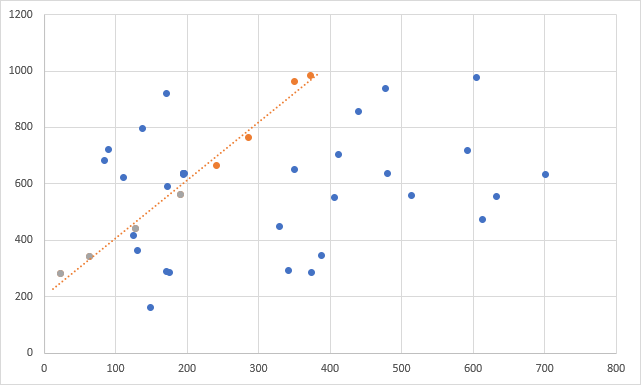
\includegraphics[width=12cm]{images/regresia1}
		  \caption{Points scattered along a trend line.}
	  \label{fig:regresia1}
	\end{figure}
	
	Let's imagine we have a single line with points scattered around it, as is illustrated in Figure \ref{fig:regresia1}. For clarity, the figure shows all points gathered from all images. To further filter out points which have almost zero probability of being real objects we introduce a threshold $T_l$ which determines a maximum distance a point can have from the line. 
	
	The distance of a point $p=(x,y)$ from the line $Am+Bn+C=0$ is calculated by using formula $$d_p=\frac{|Ax+By+C|}{\sqrt{A^2+B^2}}$$ We disregard a point if $d_p>T_l$, otherwise we process it in the next filter stage. Using only this criterion we can still be left with many false positives and thus, we extend our filter by calculating speed of every considered point. 
	
	Speed $s$ is calculated by using the well-known formula $$s=\frac{d}{{\Delta}t}$$ where $$d=\sqrt{(x_1-x_2)^2 + (y_1-y_2)^2}$$ where $(x_1,y_1)$ and $(x_2,y_2)$ are two successive points in time and $${\Delta}t=|t_1-t_2|$$ We get the time $t_{i},\ i\in\langle1,N\rangle$ where $N$ is the number of images. We treat first two objects $o_1$ and $o_2$ as the baseline - we calculate their speed and then compare speed of each successive object $o_i$ and choose the one which is closer to the baseline speed.
	
	The last stage of the filter contains calculation of angles between two successive points. Again, consider having two points represented by its positions $p_{i}=(x_i,y_i)$, $p_j=(x_j,y_j)$. We calculate angle $\theta$ between them as $$\theta=|\arctantwo(y_j-y_i, x_j-x_i)|$$ We then check whether the angle is in a predetermined threshold $T_a$. By doing this we create an imaginary 2D cone forming from each point to the plane, as is illustrated in Figure \ref{fig:regresia2}.
	
	\begin{figure}[H]
	\centering
	  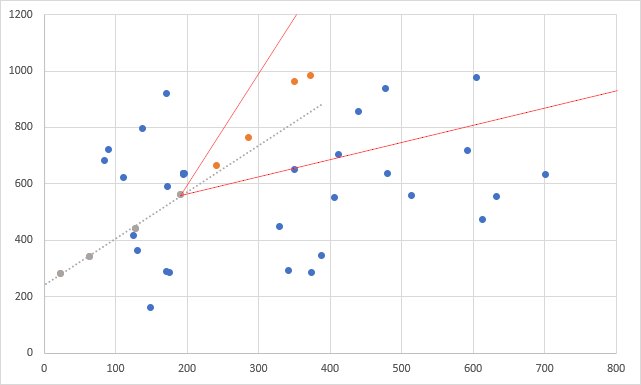
\includegraphics[width=12cm]{images/regresia2}
		  \caption{Heading of an object.}
	  \label{fig:regresia2}
	\end{figure}
	
	Only after each of these three filters has been satisfied by the currently chosen object $o_i$ and its point $p_i$, we add it to the list of potential candidates and the SLR is calculated again, containing the last added object as well. It is important to note that we add exactly one object from every image before moving to the next image.
	
	The potential candidates list now contains objects which have a high probability of being real. We touched upon every problem mentioned above - we disregarded points which are too far from the line, we correct the line by dynamically adding objects and re-calculating SLR, we filter out fake objects with nonsense speeds and angles. However, the situation when a fake object passes through all these filters is probable and is remedied by using IOD.
	
	The representation of each object $o_i$ can be specified either by the standard coordinate system in the two-dimensional Euclidean plane or by a reference system, specifically RA/Dec (see Chapter \ref{chap:object_dynamics}, Section \ref{sec:ra_dec}). The main difference and the reason why we swapped  a coordinate system for a reference system is that the RA/Dec is precise and mostly devoid of errors and deviations. The difference is best shown rather than explained - see Figure \ref{fig:regresia3}. On the left, there are shown 8 observations of the same object (an asteroid 2017\_PR25), represented in modified RA/Dec and on the right the same 8 observations, represented in the standard coordinate system. It is clearly visible that the deviation of each point in the right graph is more extreme than in the left graph. Acceleration of some of the points appears to be higher than zero - this is because the images were taken in different time intervals.
	
	\begin{figure}[H]
	\centering
	  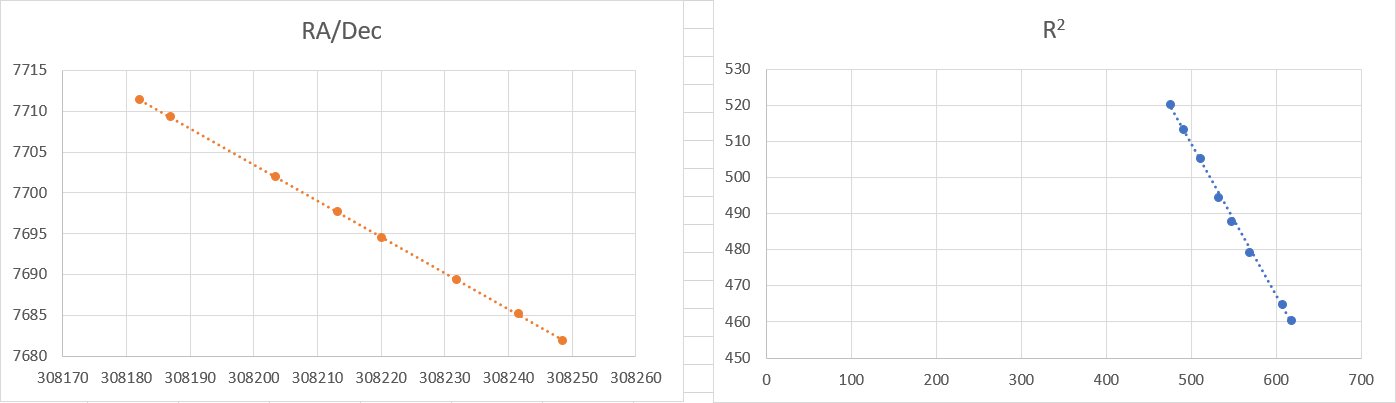
\includegraphics[width=12cm]{images/regresia3}
		  \caption{RA/Dec comparison.}
	  \label{fig:regresia3}
	\end{figure}
	
	In order to use RA/Dec in this thesis, we firstly needed to convert original values to degrees. However, due to the nature of the spherical coordinates, the points were only a hundredth, thousandth or even ten thousandth units apart. We had to modify the values by multiplying them by $10^3$ and therefore dispersing them spatially.

\section{Use of the Initial Orbit Determination algorithms}\label{sec:IDO}

	The theoretical details of IOD are described in Chapter \ref{chap:object_dynamics}, Section \ref{sec:init_orbit_det}. We used a fully functional implementation of IOD from \citep{Silha2012id}. For functioning correctly, the algorithm requires longitude and latitude in radians, altitude (in our case AGO - see Chapter \ref{chap:introduction}, Section \ref{subsec:fmpi_ago}) and RA/Dec in radians of three different objects. Then, we perform both Montenbruck and Escobal methods of IOD.

\section{Use of neural network}\label{sec:neural}

	An experimental part of this thesis is the use of a neural network. We are using a popular framework \emph{tflearn}.

\section{Hough transform}\label{sec:hough}